\documentclass{ctexart}

\usepackage{amsmath}
\usepackage{geometry}
\usepackage{booktabs}
\usepackage{graphicx}

\geometry{left = 2.0cm, right = 2.0cm , top = 3.0 cm , bottom =3.0 cm}

\begin{document}
    \title{计算物理第一次作业}
    \author{钱思天 1600011388}
    \maketitle

    \section{数值误差}
    \subsection{}
    不妨假设每次加法给出的误差为$\epsilon_i$,有:
    \begin{align*}
        &(\cdots((x_i\oplus x_2)\oplus x_3)\oplus\cdots)\oplus x_N)\\
        =&(\cdots((x_i+ x_2)(1+\epsilon_1)\oplus x_3)\oplus\cdots)\oplus x_N)\\
        =&\cdots
    \end{align*}
    略去高阶项,有:
    \begin{align*}
        &(\cdots((x_i\oplus x_2)\oplus x_3)\oplus\cdots)\oplus x_N)\\
        =&((\sum_{i=1}^N{x_i})+(x_1+x_2)\epsilon_1+\cdots+(\sum_{i=1}^N{x_i})\epsilon_{N-1})
    \end{align*}
    为进行数量级估计,取$\epsilon_i\sim \frac{\epsilon}{2}$,且将$x_i$以$\bar{|x|}$做数量级估计:
    \begin{align*}
        \epsilon_{sum}\sim\frac{(N+2)(N-1)}{2}*\frac{\epsilon}{2}\bar{|x|}
    \end{align*}
    对于均值$\bar{x}$,有:
    \begin{align*}
        \epsilon_{\bar{x}}&\sim\frac{(N+2)(N-1)}{2N}*\frac{\epsilon}{2}\bar{|x|}\\
        |\frac{\epsilon_{\bar{x}}}{\bar{x}}|&\sim\frac{(N+2)(N-1)}{2N}*\frac{\epsilon}{2}
    \end{align*}
    \subsection{}
    对于两种计算样本方差的算式,由于要避免大数相消,应该要采用第二种计算方式。
    \subsection{}
    $k=0$时:
    $$\int_0^1\frac{1}{x+5}dx=\ln{\frac{6}{5}}$$
    $k\geq1$时:
    \begin{align*}
        I_k&=\int_0^1\frac{x^k}{x+5}dx\\
        &=\frac{1}{6(k+1)}+\frac{1}{k+1}\int_0^1\frac{x^{k+1}}{(x+5)^2}dx
    \end{align*}
    可得关系式:
    $$\int_0^1\frac{x^{k+1}}{(x+5)^2}dx=(k+1)I_k-\frac{1}{6}$$
    又有:
    $$\int_0^1\frac{x^{k+1}}{(x+5)^2}dx=I_k-5\int_0^1\frac{x^{k}}{(x+5)^2}$$
    联立可得:
    $$(k+1)I_k-\frac{1}{6}=I_k-5(kI_{k-1}-\frac{1}{6})$$
    整理后有:
    $$I_k+5I_{k-1}=\frac{1}{k}$$
    如果计算$I_0$时,有一个绝对误差$\epsilon$,那么,在计算$I_k$的时候,每一步计算,都会把误差放大五倍。同时,$I_k$并不能以这么快的速度增长,相对误差会放大,因此算法不是稳定的。
    \section{矩阵的模和条件数}:
    \subsection{}
    由于矩阵的对角线全是1,上三角部分全是-1,同时是上三角矩阵,因此:
    $$det(A)=\prod_{i=1}^{N}A_{ii}=1$$
    矩阵的行列式不为零,证明矩阵不是奇异矩阵。
    \subsection{}
    考虑这样一种求逆方式,由于
    $$if:BA=I,then:BI=A^{-1}$$
    即,如果我对矩阵$A$求逆,假设一系列基本变换(即线性变换,i.e.调换行顺序或调换列顺序或将一行/列乘以一定倍数加到另一行/列上)能使$A$变为单位阵,那么,同样的一系列操作作用在单位阵$I$上,就可以变为$A$的逆矩阵。
    \par
    按照这一流程,下考虑将$A$变成单位阵的基本变换组合:
    $$
        A=
        \left(
            \begin{matrix}
                1&-1&\cdots&-1\\
                0&1&\cdots&-1\\
                \vdots&\vdots&\ddots&\vdots\\
                0&\cdots&\cdots&1
            \end{matrix}
        \right)
    $$
    因而将$A$变成单位阵$I$,首先把第一列加到之后的每一列上,然后把第二列加到之后的每一列上……
    \par
    将相同的操作作用在单位阵上,可以得到A的逆矩阵:
    $$
        A^{-1}=
        \left(
            \begin{matrix}
                1&1&\cdots&2^{n-2}\\
                0&1&\cdots&2^{n-3}\\
                \vdots&\vdots&\ddots&\vdots\\
                0&\cdots&\cdots&1
            \end{matrix}
        \right)
    $$
    将具体的矩阵元表示出来,就是:
    \begin{align*}
        A^{-1}_{ii}&=1;\\
        A^{-1}_{ij}&=0,j<i\\
        A^{-1}_{ij}&=2^{j-i-1},j>i;
    \end{align*}
    \subsection{}
    当$p\to\infty$时,矩阵$p-$模的定义式为:
    $$||A||_{\infty}=\lim_{p\to\infty}{\sup_{x\neq0}{\frac{||Ax||_p}{||x||_p}}}$$
    向量的$\infty$模取值如下:
    $$||v||_{\infty}=\max{(|v_i|)}$$
    因此,对于矩阵的无穷模,首先考虑这样的诱导向量$x$的集合$X$:
    $$X=\{x;\forall 1\leq i \leq N,|x_i|=1\}$$
    则有$|x|_{\infty}=1$,又有:我们总可以选择各$x_i$的符号与$A$的每一行中各个元素匹配,故有:
    $$\forall 1\leq i \leq N,\sum_{j=1}^{N}{A_{ij}x_j}\leq\sum_{j=1}^{N}{|A_{ij}|}$$
    总能适当选取$x\in X$使得等号成立。可得:
    $$\sup_{x\in X}{||Ax||_{\infty}}=\max_{1\leq i \leq N}{\sum_{j=1}^{N}{|A_{ij}|}}$$
    即:
    $$\sup_{x\in X}\frac{||Ax||_{\infty}}{||x||_\infty}=\max_{1\leq i \leq N}{\sum_{j=1}^{N}{|A_{ij}|}}$$
    对于任意的各分量绝对值相等的诱导矢量$y$可按上述过程计算,只不过$||y||_\infty$和$||Ay||_\infty$都乘上一个因子,比值的上确界不变。
    
    \par
    对于各分量不都相等的诱导矢量$z$,不妨设分量绝对值最大值为$M$,即$||z||_\infty=M$。对于$Az$的各个分量,有:
    \begin{align*}
    &|\sum_{j=1}^{N}{A_{ij}{z_j}}|\\
    \leq&\sum_{j=1}^{N}{|A_{ij}{z_j}|}\\
    \leq&\sum_{j=1}^{N}{|A_{ij}M|}\\
    =&M\sum_{j=1}^N{|A_{ij}|}
    \end{align*}
    有
    $$\sup_{||z||_\infty=M}\frac{||Az||_{\infty}}{||z||_\infty}\leq\max_{1\leq i \leq N}{\sum_{j=1}^{N}{|A_{ij}|}}$$
    \par
    综上,有:
    $$\sup_{x}\frac{||Ax||_{\infty}}{||x||_\infty}=\max_{1\leq i \leq N}{\sum_{j=1}^{N}{|A_{ij}|}}$$
    证毕。
    \subsection{}
    对于矢量$x$,其欧式模可以用内积$(,)$的形式给出:
    $$||x||_2=\sqrt{(x,x)}$$
    那么,对于幺正矩阵$U$,对任意矢量$x$,都有:
    \begin{align*}
        &||Ux||_2\\
        =&\sqrt{(Ux,Ux)}\\
        =&\sqrt{(U^{\dagger}Ux,x)}\\
        =&\sqrt{(x,x)}
    \end{align*}
    换而言之,$$||U||_2=1$$同理,$$||U^{\dagger}||_2=1$$
    同时,由于$\forall x$有:
    \begin{align*}
        &||UAx||_2\\
        =&\sqrt{(UAx,UAx)}\\
        =&\sqrt{(U^{\dagger}UAx,Ax)}\\
        =&\sqrt{(Ax,Ax)}\\
        =&||Ax||_2
    \end{align*}
    也可得$||UA||_2=||A||_2$,对条件数有$K_2(A)=K_2(UA)$。
    \subsection{}
    \begin{align*}
        &K_\infty(A)\\
        =&||A||_\infty*||A^{-1}||_\infty\\
        =&n2^n
    \end{align*}
    \section{Hilbert Matrix}
    \subsection{}
    原问题为:
    $$\min_{\vec{c}}D=\min_{\forall c_i}{\int_0^1(\sum_{i=1}^{n}c_ix^{i-1}-f(x))^2}$$
    可得关系式:
    $$\frac{\partial D}{\partial c_i}=0$$
    即:
    $$\int_0^1dx\sum_{j=1}^{n}c_jx^{j-1}*x^{i-1}=\int_0^1dxf(x)x^{i-1}$$
    换而言之:
    $$H_{ij}=\int_0^1x^{i+j-2}=\frac{1}{i+j-1}$$
    $$b_i=\int_0^1f(x)x^{i-1}$$
    \subsection{}
    对任意向量$v_i$,则二次型:
    \begin{align*}
        &v^THv\\
        =&\sum_{i=1}^{N}\sum_{j=1}^{N}{\frac{v_iv_j}{i+j-1}}\\
        =&\int_0^1\sum_{i,j}t^{i+j-2}*v_iv_jdt\\
        =&\int_0^1(\sum_{i}{v_it^{i-1}})^2dt\geq0
    \end{align*}
    即Hilbert Matrix是正定的。
    \subsection{}
    为了估算Hilbert Matrix的行列式,根据计算式,取对数,有:
    $$\ln{(\det{(H_n)})}=4\sum_{i=2}^{n-1}{\ln{i!}}-\sum_{j=2}^{2n-1}{\ln{j!}}$$
    $n>1$时利用斯特林公式$n!=\sqrt{2\pi n}{(\frac{n}{e})^n}$(相关讨论见附录),可以得到估计值如下:
    \begin{table}[htbp]
        \centering
        \begin{tabular}{rrr}
            \toprule
             n &     $\ln{|H_n|}$ &           $|H_n|$ \\
            \midrule
            1 &    0.000000 &  1.000000e+00 \\
            2 &   -2.415888 &  8.928801e-02 \\
            3 &   -7.736772 &  4.364781e-04 \\
            4 &  -15.759086 &  1.431911e-07 \\
            5 &  -26.516797 &  3.047203e-12 \\
            6 &  -40.024225 &  4.146675e-18 \\
            7 &  -56.288751 &  3.581839e-25 \\
            8 &  -75.314679 &  1.955467e-33 \\
            9 &  -97.104737 &  6.728970e-43 \\
            10 & -121.660763 &  1.456806e-53 \\
            \bottomrule
            \end{tabular}
    \end{table}
    \subsection{}
    利用两种不同方法解方程得到的解如下:
    \begin{enumerate}
        \item n=1
        \begin{enumerate}
            \item GEM\newline
            ( 1.0000 )
            \item Cholesky\newline
            ( 1.0000 )
        \end{enumerate}
        \item n=2
        \begin{enumerate}
            \item GEM\newline
            ( -2.0000, 6.0000 )
            \item Cholesky\newline
            ( -2.0000, 6.0000 )
        \end{enumerate}
        \item n=3
        \begin{enumerate}
            \item GEM\newline
            ( 3.0000, -24.0000, 30.0000 )
            \item Cholesky\newline
            ( 3.0000, -24.0000, 30.0000 )
        \end{enumerate}
        \item n=4
        \begin{enumerate}
            \item GEM\newline
            ( -4.0000, 60.0000, -180.0000, 140.0000 )
            \item Cholesky\newline
            ( -4.0000, 60.0000, -180.0000, 140.0000 )
        \end{enumerate}
        \item n=5
        \begin{enumerate}
            \item GEM\newline
            ( 5.0000, -120.0000, 630.0000, -1120.0000, 630.0000 )
            \item Cholesky\newline
            ( 5.0000, -120.0000, 630.0000, -1120.0000, 630.0000 )
        \end{enumerate}
        \item n=6
        \begin{enumerate}
            \item GEM\newline
            ( -6.0000, 210.0000, -1680.0000, 5040.0000, -6300.0000, 2772.0000 )
            \item Cholesky\newline
            ( -6.0000, 210.0000, -1680.0000, 5040.0000, -6300.0000, 2772.0000 )
        \end{enumerate}
        \item n=7
        \begin{enumerate}
            \item GEM\newline
            ( 7.0000, -336.0000, 3780.0000, -16800.0001, 34650.0001, -33264.0001, 12012.0000 )
            \item Cholesky\newline
            ( 7.0000, -336.0000, 3780.0000, -16800.0001, 34650.0001, -33264.0001, 12012.0000 )
        \end{enumerate}
        \item n=8
        \begin{enumerate}
            \item GEM\newline
            ( -8.0000, 504.0000, -7559.9998, 46199.9991, -138599.9973, 216215.9960, -168167.9970, 51479.9991 )
            \item Cholesky\newline
            ( -8.0000, 504.0000, -7559.9998, 46199.9989, -138599.9969, 216215.9954, -168167.9966, 51479.9990 )
        \end{enumerate}
        \item n=9
        \begin{enumerate}
            \item GEM\newline
            ( 8.9999, -719.9962, 13859.9351, -110879.5319, 450448.2691, -1009004.4428, 1261255.8924, -823677.5075, 218789.3817 )
            \item Cholesky\newline
            ( 8.9999, -719.9957, 13859.9269, -110879.4726, 450448.0491, -1009003.9891, 1261255.3671, -823677.1880, 218789.3023 )
        \end{enumerate}
        \item n=10
        \begin{enumerate}
            \item GEM\newline
            ( -9.9980, 989.8301, -23756.3837, 240207.1395, -1261103.3278, 3783349.4733, -6726013.8839, 7000597.8401, -3937861.9782, 923701.2873 )
            \item Cholesky\newline
            ( -9.9938, 989.4539, -23748.1253, 240130.1994, -1260728.8024, 3782302.1150, -6724270.1513, 6998891.2685, -3936956.0905, 923500.1211 )
        \end{enumerate}
    \end{enumerate}
    可以看出,两者的解有细微的差别,我认为用GEM给出的解更好,原因中重要的一点是我自己实现的牛顿法开方\par
    若不考虑开方引起的误差,我认为Cholesky应该可以给出更好的解,原因是输出前几个解答(此时牛顿法给出的平方根也更准确)的高精度数值时,会发现GEM的偏差较大。关于这一点,我认为是由于GEM加减中的舍入误差导致。
\newpage{}
    \appendix{附录:关于斯特林公式近似的有效性}
    \newline
   
    \begin{figure}[h]
        \centering
        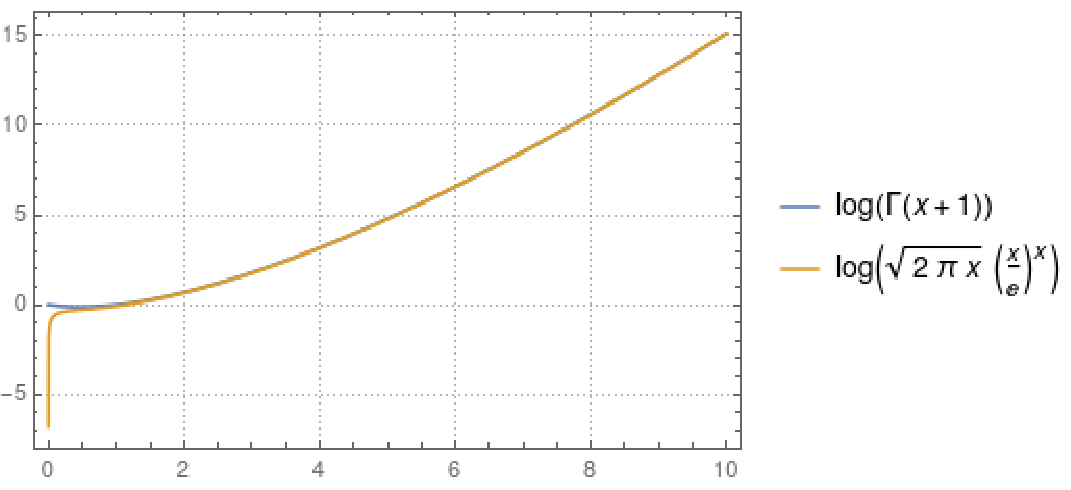
\includegraphics[width=\textwidth]{Stirling.pdf}
        \caption{利用Mathematica所绘制的Stirling近似和直接计算阶乘对数的比较}
        \label{fig:1}
    \end{figure}
    如图所见,当$x\geq2$时,Stirling近似可以给出很好的近似,而$x=1$时,对数是零,事实上原式中我们可以直接从$n=2$求和。
\end{document}